\documentclass[conference]{IEEEtran}
\usepackage[T1]{fontenc}
\usepackage[utf8]{inputenc}
\usepackage[spanish,es-tabla,es-nodecimaldot,es-noshorthands]{babel}
\usepackage{cite}
\usepackage{amsmath,amssymb,amsfonts}
\usepackage{graphicx}
\usepackage{textcomp}
\usepackage{xcolor}
\usepackage{booktabs}
\usepackage{url}
\usepackage{tikz}
\usetikzlibrary{positioning,arrows.meta}
\usepackage[colorlinks=true,urlcolor=blue,linkcolor=black,citecolor=black]{hyperref} % enlaces clicables; va al final
\renewcommand\IEEEkeywordsname{Palabras clave}

\begin{document}

\title{Clasificación de calidad y tamaño de frutas con visión por computador: de un dataset público a fotos propias}

\author{\IEEEauthorblockN{Jaime Muñoz}
\IEEEauthorblockA{\textit{Ingeniería de Sistemas} \\
\textit{Universidad Icesi}\\
Cali, Colombia}
\and
\IEEEauthorblockN{Andres Felipe Lopez}
\IEEEauthorblockA{\textit{Ingeniería de Sistemas} \\
\textit{Universidad Icesi}\\
Cali, Colombia}
}

\maketitle

\begin{abstract}
En las plazas de mercado la fruta se separa por calidad a ojo, y el resultado depende de quién lo haga. Construimos un sistema que, a partir de la foto de una fruta sobre un fondo uniforme, predice su calidad (good, regular o bad) y una clase de tamaño. Usamos 13\,696 imágenes de un dataset público y 850 archivos de fotos tomadas por nosotros, que corresponden a 714 tomas distintas. Comparamos seis clasificadores entrenados sobre 62 características de color, textura y forma con una red convolucional pequeña entrenada desde cero, y evaluamos con una partición que deja todas las fotos de una misma fruta en el mismo conjunto. En las imágenes del dataset público los mejores modelos obtienen un F1 macro de 0.96 a 0.97; en nuestras fotos los mejores llegan a 0.86 y la red convolucional a 0.59. Encontramos dos fugas de datos que inflaban las métricas en nuestras fotos: ráfagas de fotos casi idénticas y copias rotadas de una misma foto. El tamaño, estimado con el diámetro equivalente del contorno, es estable entre tomas de la misma fruta, pero la clase cambia con facilidad cerca de los límites entre tamaños. La diferencia entre las dos fuentes de imágenes limita el sistema más que la elección del modelo.
\end{abstract}

\begin{IEEEkeywords}
calidad de frutas, visión por computador, aprendizaje automático, cambio de dominio, fuga de datos
\end{IEEEkeywords}

{\small\raggedright\noindent\textbf{Video de presentación:} \href{https://www.youtube.com/watch?v=JPqTPEJS1IE}{youtube.com/watch?v=JPqTPEJS1IE}\\
\textbf{Código:}\\
\href{https://github.com/byrejaxxmodz/apo3-fruit-quality-classification}{github.com/byrejaxxmodz/apo3-fruit-quality-classification}\par}

\section{Introducción}

Según la FAO, cerca del 14\,\% de los alimentos que se producen en el mundo se pierde entre la cosecha y la venta al por menor \cite{fao2019}. En Colombia, el Departamento Nacional de Planeación estimó en 9.76 millones de toneladas al año la pérdida y el desperdicio de alimentos, alrededor del 34\,\% de lo disponible para consumo humano \cite{dnp2016}. Una parte de esa pérdida ocurre en la comercialización, donde la fruta se clasifica a mano. En una plaza de mercado esa clasificación la hace una persona mirando cada pieza; es lenta, y dos vendedores pueden no estar de acuerdo sobre la misma fruta.

Automatizar esa decisión con una cámara barata es un problema de visión por computador conocido. Existen datasets públicos con fotos de frutas etiquetadas por calidad, como FruitNet \cite{meshram2022}, y trabajos que reportan exactitudes cercanas al 99.7\,\% sobre él \cite{morshed2022}. Esas cifras se obtienen con fotos del mismo origen en entrenamiento y prueba. No sabíamos si se mantendrían con fotos tomadas por nosotros, con otros celulares, otra luz y variedades locales; la granadilla, por ejemplo, no está en FruitNet.

El objetivo fue construir un sistema que reciba la foto de una fruta y devuelva su calidad en tres clases y una clase de tamaño, y medir qué tan bien funciona con fotos propias. Los aportes son: un conjunto de fotos propias con tres clases de calidad, incluida regular, que el dataset público no tiene; una comparación entre clasificadores clásicos sobre características manuales y una red convolucional pequeña, con resultados por fuente, intervalos de confianza y pruebas pareadas; la detección de dos fugas de datos y de imágenes generadas con IA; y una aplicación web de demostración. El código y el video están enlazados debajo de las palabras clave.

\section{Fundamentos teóricos}

\subsection{Formulación del problema}
Dada la foto $I\in[0,255]^{H\times W\times 3}$ de una fruta, el sistema calcula dos funciones: $f_q(I)=\hat y_q\in\mathcal{Q}=\{$good, regular, bad$\}$, la calidad, y $f_s(I)=\hat y_s\in\mathcal{S}=\{$pequeño, mediano, grande$\}$, el tamaño. La función $f_s$ no se aprende, sino que se calcula con la máscara de segmentación (Sección~\ref{sec:seg}). La función $f_q$ se aprende de $N$ ejemplos etiquetados $(I_i,y_i)$. En los modelos clásicos $f_q=h_\theta\circ\phi$, donde $\phi(I)=\mathbf{x}\in\mathbb{R}^{62}$ es el vector de características de la Sección~\ref{sec:desc} y $h_\theta$ el clasificador. En la CNN la representación también se aprende. Salvo KNN, que no se entrena, y Random Forest, que construye cada árbol reduciendo la impureza de Gini, los modelos ajustan sus parámetros minimizando el riesgo empírico ponderado
\begin{equation}
\hat\theta=\arg\min_\theta\;\frac{1}{N}\sum_{i=1}^{N} w_{y_i}\,\ell\big(y_i,h_\theta(\mathbf{x}_i)\big)+\Omega(\theta),
\label{eq:erm}
\end{equation}
donde $\ell$ es la pérdida de cada modelo (bisagra en el SVM, entropía cruzada en la regresión logística, XGBoost y la CNN) y $\Omega$ su regularización. El peso $w_k=N/(KN_k)$ de la clase $k$, que tiene $N_k$ ejemplos, compensa el desbalance en los modelos que admiten pesos. Los hiperparámetros, como $C$ y $\gamma$ en el SVM, se eligen maximizando el F1 macro en validación cruzada agrupada.

El problema es complejo por cuatro razones. Dentro de cada clase hay mucha variación por variedad, madurez, luz y cámara. La frontera de la clase regular es subjetiva. Esa clase tiene pocos ejemplos y viene de una sola fuente, lo que abre la puerta a atajos. Y el tamaño real no se puede recuperar de una foto sin escala.

\subsection{Segmentación y tamaño}
\label{sec:seg}
Las fotos tienen una sola fruta sobre un fondo neutro, que tiene saturación cercana a cero en el espacio HSV; la fruta tiene saturación alta. El histograma del canal de saturación $S$ es entonces bimodal, y el método de Otsu \cite{otsu1979} elige el umbral que maximiza la varianza entre las dos clases de píxeles:
\begin{equation}
t^* = \arg\max_t \; \omega_0(t)\,\omega_1(t)\,[\mu_0(t)-\mu_1(t)]^2,
\end{equation}
donde $\omega_i$ es la proporción de píxeles a cada lado del umbral y $\mu_i$ su media. Una apertura y un cierre morfológicos limpian la máscara. Con el área $A$ de la máscara se calcula el diámetro equivalente y se normaliza por el lado menor de la imagen:
\begin{equation}
d_{eq}=\sqrt{4A/\pi}, \qquad d_{norm}=d_{eq}/\min(H,W).
\end{equation}
Con el modelo de cámara estenopeica, $d_{norm}$ es proporcional a $D f / Z$, donde $D$ es el diámetro real, $f$ la distancia focal y $Z$ la distancia a la cámara. Sin una distancia fija o un objeto de referencia, $d_{norm}$ solo permite comparar frutas fotografiadas en las mismas condiciones.

\subsection{Descriptores de color y textura}
\label{sec:desc}
El color se describe con histogramas normalizados de los canales H, S y V, que separan el tono de la iluminación, y con la media, la desviación y la asimetría de cada canal Lab; una mancha oscura sesga la distribución de L. La textura se describe con patrones binarios locales uniformes (LBP) \cite{ojala2002}, que codifican cómo se compara cada píxel con sus vecinos, y con cuatro estadísticos de la matriz de co-ocurrencia de niveles de gris (GLCM) \cite{haralick1973}: contraste, homogeneidad, energía y correlación. Se añaden la fracción de píxeles oscuros y marrones como indicio de defectos, y la circularidad, la solidez y la relación de aspecto del contorno.

\subsection{Clasificadores}
La máquina de vectores de soporte (SVM) \cite{cortes1995} busca el hiperplano de máximo margen; con un kernel RBF, $K(\mathbf{x},\mathbf{x}')=e^{-\gamma\|\mathbf{x}-\mathbf{x}'\|^2}$, la frontera puede ser no lineal. K vecinos más cercanos (KNN) asigna la clase mayoritaria entre los $k$ ejemplos de entrenamiento más cercanos. Random Forest \cite{breiman2001} promedia árboles entrenados sobre muestras bootstrap, y XGBoost \cite{chen2016} suma árboles poco profundos, cada uno ajustado al error de los anteriores. Usamos además regresión logística multinomial y un perceptrón multicapa (MLP).

La red convolucional (CNN) aprende sus propios filtros. Cada bloque aplica una convolución $3\times3$, normalización por lotes \cite{ioffe2015}, ReLU y max-pooling. Al final, el promedio global por canal (global average pooling) \cite{lin2014} reemplaza a la capa densa grande y reduce los parámetros, lo que importa cuando hay pocos datos. Se entrena con entropía cruzada ponderada por clase, Adam \cite{kingma2015}, una tasa de aprendizaje con decaimiento coseno \cite{loshchilov2017} y dropout \cite{srivastava2014}.

\subsection{Evaluación}
Las clases están desbalanceadas, así que usamos el F1 macro, que pesa igual a las tres clases:
\begin{equation}
F1_k=\frac{2P_kR_k}{P_k+R_k}, \qquad F1_{macro}=\frac{1}{K}\sum_{k=1}^{K}F1_k,
\end{equation}
donde $P_k$ y $R_k$ son la precisión y el recall de la clase $k$. Si fotos casi idénticas de una misma fruta quedan unas en entrenamiento y otras en prueba, el modelo las reconoce de memoria y la métrica de prueba sobreestima su desempeño; es una forma de fuga de datos \cite{kaufman2012}. Por eso la partición y la validación cruzada se hacen por grupos de fotos de la misma fruta.

Con pocas fotos de prueba, una métrica puntual dice poco sin su incertidumbre. Para proporciones como el recall usamos el intervalo de Wilson \cite{wilson1927}, y para el F1 macro un bootstrap \cite{efron1993} que remuestrea grupos de fotos y no fotos sueltas. Para comparar dos modelos sobre las mismas imágenes usamos la prueba exacta de McNemar \cite{mcnemar1947,dietterich1998}, que solo cuenta las imágenes en que un modelo acierta y el otro falla, con la corrección de Holm \cite{holm1979} por hacer muchas comparaciones.

\section{Metodología}

Seguimos las fases de CRISP-DM \cite{chapman2000}. La Fig.~\ref{fig:flujo} resume el proceso tal como lo hicimos, incluida la vuelta atrás que obligó a corregir la partición.

\begin{figure*}[t]
\centering
\resizebox{\textwidth}{!}{%
\begin{tikzpicture}[
  caja/.style={draw, rounded corners=2pt, align=center, font=\footnotesize, text width=2.55cm, inner sep=3pt},
  alta/.style={caja, minimum height=3.1cm},
  baja/.style={caja, minimum height=0.9cm},
  fase/.style={font=\footnotesize\itshape},
  flecha/.style={-{Stealth[length=1.8mm]}, semithick}]
\node[font=\footnotesize, text width=17.5cm, align=center] at (8.0,2.6)
  {\textit{Comprensión del negocio:} separar fruta good, regular y bad y estimar su tamaño a partir de una foto tomada con un celular o una cámara web};
\node[alta] (datos) at (0,0) {Kaggle (FruitNet):\\13\,696 imágenes\\[3pt] Fotos propias:\\850 archivos,\\714 tomas distintas};
\node[alta] (control) at (3.2,0) {30 imágenes generadas con IA: excluidas\\[3pt] Ráfagas y copias rotadas: en el grupo de su original};
\node[alta] (prep) at (6.4,0) {Segmentación con HSV y Otsu\\[3pt] Recorte de 128$\times$128 sin fondo\\[3pt] Partición agrupada 70/15/15};
\node[baja] (ml) at (9.6,1.1) {62 características: SVM, KNN, RF, LR, MLP y XGBoost};
\node[baja] (cnn) at (9.6,0) {CNN desde cero, 102 mil parámetros};
\node[baja] (tam) at (9.6,-1.1) {Tamaño: $d_{norm}$ y terciles por fruta};
\node[alta] (eval) at (12.8,0) {F1 macro por fuente\\[3pt] IC 95\,\% y McNemar\\[3pt] Fiabilidad del tamaño entre tomas};
\node[alta] (app) at (16.0,0) {App web: foto por archivo o cámara; muestra máscara, probabilidades y tamaño};
\node[fase, above=2pt of datos] {Datos};
\node[fase, above=2pt of control] {Calidad de los datos};
\node[fase, above=2pt of prep] {Preparación};
\node[fase, above=2pt of ml] {Modelado};
\node[fase, above=2pt of eval] {Evaluación};
\node[fase, above=2pt of app] {Despliegue};
\draw[flecha] (datos) -- (control);
\draw[flecha] (control) -- (prep);
\foreach \m in {ml,cnn,tam} {
  \draw[flecha] (prep.east) -- (\m.west);
  \draw[flecha] (\m.east) -- (eval.west);
}
\draw[flecha] (eval) -- (app);
\draw[flecha, dashed] (eval.south) -- ++(0,-0.5) -| node[pos=0.25, below, font=\footnotesize]
  {fugas de datos encontradas al evaluar: se corrige la partición y se repite} (control.south);
\end{tikzpicture}}
\caption{Proceso seguido, organizado por fases de CRISP-DM. La flecha punteada es la iteración que hicimos dos veces, al encontrar cada fuga de datos.}
\label{fig:flujo}
\end{figure*}

\subsection{Datos}
La fuente principal es el dataset Fruit Quality Classification de Kaggle \cite{park2024}, una copia de FruitNet \cite{meshram2022}: seis frutas fotografiadas en India, en carpetas good, bad y mixed. La carpeta mixed tiene varias frutas por foto y no la usamos. La granada buena tenía 5\,940 fotos y las demás carpetas unas 1\,100, así que tomamos como máximo 1\,200 por carpeta, con una semilla fija. Las fotos propias las tomamos con nuestros celulares, una fruta por foto sobre fondo liso, y cada foto se guardó en la carpeta de su clase siguiendo una definición escrita: good, sin defectos visibles; regular, apta para el consumo pero con defectos leves (manchas en menos del 10\,\% de la superficie, un golpe leve o madurez avanzada); bad, no apta para la venta (podredumbre, moho, piel rota o manchas en más del 30\,\%). La Tabla~\ref{tab:datos} resume los conteos.

\begin{table}[t]
\caption{Imágenes por fruta, fuente y clase de calidad}
\label{tab:datos}
\centering
\footnotesize
\setlength{\tabcolsep}{4pt}
\begin{tabular*}{\columnwidth}{@{\extracolsep{\fill}}lrrrrr}
\toprule
 & \multicolumn{2}{c}{Kaggle} & \multicolumn{3}{c}{Fotos propias} \\
\cmidrule(lr){2-3}\cmidrule(lr){4-6}
Fruta & good & bad & good & regular & bad \\
\midrule
Manzana & 1\,149 & 1\,141 & 169 & 24 & 3 \\
Banano & 1\,113 & 1\,087 & 46 & 66 & 40 \\
Guayaba & 1\,152 & 1\,129 & 31 & 62 & 103 (24) \\
Lima & 1\,094 & 1\,085 & 70 & 39 (5) & 30 (7) \\
Naranja & 1\,200 & 1\,159 & 86 & 36 & 27 \\
Granada & 1\,200 & 1\,187 & -- & -- & -- \\
Granadilla & -- & -- & -- & 11 & 7 \\
\midrule
Total & 6\,908 & 6\,788 & 402 & 238 (204) & 210 (108) \\
\bottomrule
\end{tabular*}
\par\smallskip
\parbox{\columnwidth}{\scriptsize Entre paréntesis, tomas distintas cuando hay copias rotadas de una misma foto.}
\end{table}

\subsection{Control de calidad de los datos}
Revisar los datos antes de entrenar cambió los resultados más que cualquier ajuste de hiperparámetros. En la carpeta compartida encontramos 30 imágenes generadas con IA, 27 de ellas en la carpeta de manzanas bad; las detectamos por los metadatos de procedencia que dejan los generadores (C2PA e IPTC) \cite{c2pa} y las excluimos. También encontramos 148 archivos que eran copias rotadas o volteadas de solo 33 fotos de guayaba y lima. Esas copias se pueden usar para entrenar, pero cada una debe ir al mismo conjunto que su original. Por último, las imágenes de Kaggle conservan en sus metadatos EXIF las coordenadas GPS de donde se tomaron, así que no las redistribuimos.

La clase regular solo existe en nuestras fotos. Un modelo podría aprender entonces que una foto de celular colombiano es regular sin mirar la fruta. Por eso todos los resultados se reportan también por fuente.

\subsection{Preparación}
Cada foto se reduce a 512 píxeles en su lado mayor, se segmenta y se recorta en un cuadro de $128\times128$ con el fondo en negro, para que el modelo no vea el entorno. La clase de tamaño se asigna con los terciles de $d_{norm}$ por fuente y por fruta: una naranja grande no mide lo mismo que una lima grande, y en Kaggle la fruta ocupa más cuadro que en nuestras fotos. No la etiquetamos a ojo, porque sin un objeto de referencia una persona tampoco puede saber el tamaño real de la fruta en la foto. Con una regla escrita, todas las fotos se miden con el mismo criterio, y la regla se valida con la repetibilidad entre tomas de la misma fruta (Sección~\ref{sec:resultados}).

La partición es 70/15/15, estratificada por calidad y agrupada. Dos recortes de la misma carpeta quedan en el mismo grupo si la similitud coseno entre sus miniaturas de $32\times32$ supera 0.95, y además cada copia rotada se une al grupo de su original. En la primera versión del proyecto la partición era aleatoria: 53 de las 91 fotos propias de prueba tenían una gemela casi idéntica en entrenamiento, y el F1 macro del SVM en fotos propias bajó de 0.97 a 0.75 al agrupar. Más adelante encontramos que las copias rotadas no se parecían lo suficiente para caer en el mismo grupo: 17 de las 28 fotos bad propias de prueba tenían una copia suya en entrenamiento. Los resultados de este informe usan la partición corregida, con 111 fotos propias en prueba (59 good, 23 regular y 29 bad).

\subsection{Modelado}
Las características diseñadas describen directamente lo que separa las clases: color, manchas y textura. Además necesitan menos datos que una red, que debe aprender esa representación por sí misma. Por eso son la base, y la CNN sirve de comparación. Descartamos tres alternativas:
\begin{itemize}
\item Un detector de objetos como YOLO: cada foto tiene una sola fruta, y habría que anotar cajas.
\item Una red de segmentación como U-Net: necesita máscaras hechas a mano, y con fondo uniforme Otsu es suficiente.
\item El aprendizaje por transferencia: la guía del curso lo permite, pero recomienda entrenar desde cero. Queda como trabajo futuro.
\end{itemize}

Los clasificadores clásicos se entrenaron con un pipeline de estandarización y clasificador, de modo que la media y la desviación se calculan solo con los datos de entrenamiento de cada pliegue. Los hiperparámetros de cada modelo se eligieron con búsqueda en rejilla y validación cruzada agrupada de cinco pliegues, maximizando el F1 macro. El desbalance se compensó con los pesos $w_k$ de (\ref{eq:erm}).

La CNN tiene tres bloques convolucionales de 32, 64 y 128 filtros, promedio global, dropout y dos capas densas, con 101\,923 parámetros. Durante el entrenamiento cada recorte se voltea, se rota múltiplos de $90^\circ$ y se le varían la saturación y el brillo al azar. Exploramos ocho configuraciones (tasa de aprendizaje $10^{-3}$ o $3\cdot10^{-4}$, dropout 0.3 o 0.5, y dos anchos de red) con 35 épocas como máximo y parada temprana según el F1 de validación. Ganó la tasa $3\cdot10^{-4}$ con dropout 0.5 y la red ancha. La búsqueda se hizo con la partición anterior; con la partición corregida reentrenamos solo esa configuración. Usamos scikit-learn \cite{pedregosa2011}, XGBoost y PyTorch \cite{paszke2019}, con la GPU de un portátil Apple.

\subsection{Evaluación}
El conjunto de prueba se usó una sola vez, al final. Reportamos el F1 macro global, el de cada fuente y el recall de las clases regular y bad en nuestras fotos, comparados con una línea base que siempre predice la clase mayoritaria. Los intervalos de confianza son del 95\,\%, con 2\,000 remuestreos por grupos para el F1.

\subsection{Despliegue}
La aplicación, hecha con Streamlit, recibe una foto subida o tomada con la cámara del equipo, muestra la máscara de segmentación, las probabilidades de cada clase y la clase de tamaño, y avisa cuando la segmentación falla. Corre en la CPU de un portátil, a unos 75~ms por foto con los modelos clásicos.

\section{Resultados}
\label{sec:resultados}

\subsection{Clasificación de calidad}
La Tabla~\ref{tab:resultados} resume el desempeño en prueba y la Fig.~\ref{fig:ic} muestra los intervalos de confianza por fuente. En las imágenes de Kaggle, KNN, SVM, MLP y XGBoost obtienen entre 0.96 y 0.97 de F1 macro. En nuestras fotos todos bajan entre 0.10 y 0.30 puntos.

\begin{table}[t]
\caption{F1 macro y recall en prueba. CV: validación cruzada agrupada (para la CNN, F1 de validación). IC del 95\,\% por bootstrap de grupos}
\label{tab:resultados}
\centering
\footnotesize
\setlength{\tabcolsep}{3pt}
\begin{tabular}{lcccccc}
\toprule
 & & & \multicolumn{4}{c}{Fotos propias} \\
\cmidrule(lr){4-7}
Modelo & CV & Kaggle & F1 & IC 95\,\% & Reg. & Bad \\
\midrule
KNN ($k=3$) & 0.90 & 0.96 & 0.86 & [0.75, 0.94] & 0.91 & 0.76 \\
SVM RBF ($C=10$) & 0.92 & 0.97 & 0.86 & [0.74, 0.95] & 0.87 & 0.72 \\
MLP (128, 64) & 0.89 & 0.96 & 0.85 & [0.73, 0.93] & 0.78 & 0.83 \\
XGBoost & 0.92 & 0.97 & 0.82 & [0.71, 0.91] & 0.57 & 0.93 \\
Random Forest & 0.86 & 0.94 & 0.69 & [0.55, 0.79] & 0.30 & 0.83 \\
Reg. logística & 0.72 & 0.89 & 0.60 & [0.42, 0.72] & 0.87 & 0.59 \\
CNN & 0.74 & 0.88 & 0.59 & [0.46, 0.70] & 0.43 & 0.62 \\
Clase mayoritaria & -- & 0.32 & 0.23 & [0.18, 0.27] & 0.00 & 0.00 \\
\bottomrule
\multicolumn{7}{p{0.95\columnwidth}}{\scriptsize Reg. y Bad: recall de esas clases en fotos propias. Prueba: 1\,987 imágenes de Kaggle y 111 propias de 62 frutas físicas.}
\end{tabular}
\end{table}

\begin{figure*}[t]
\centering
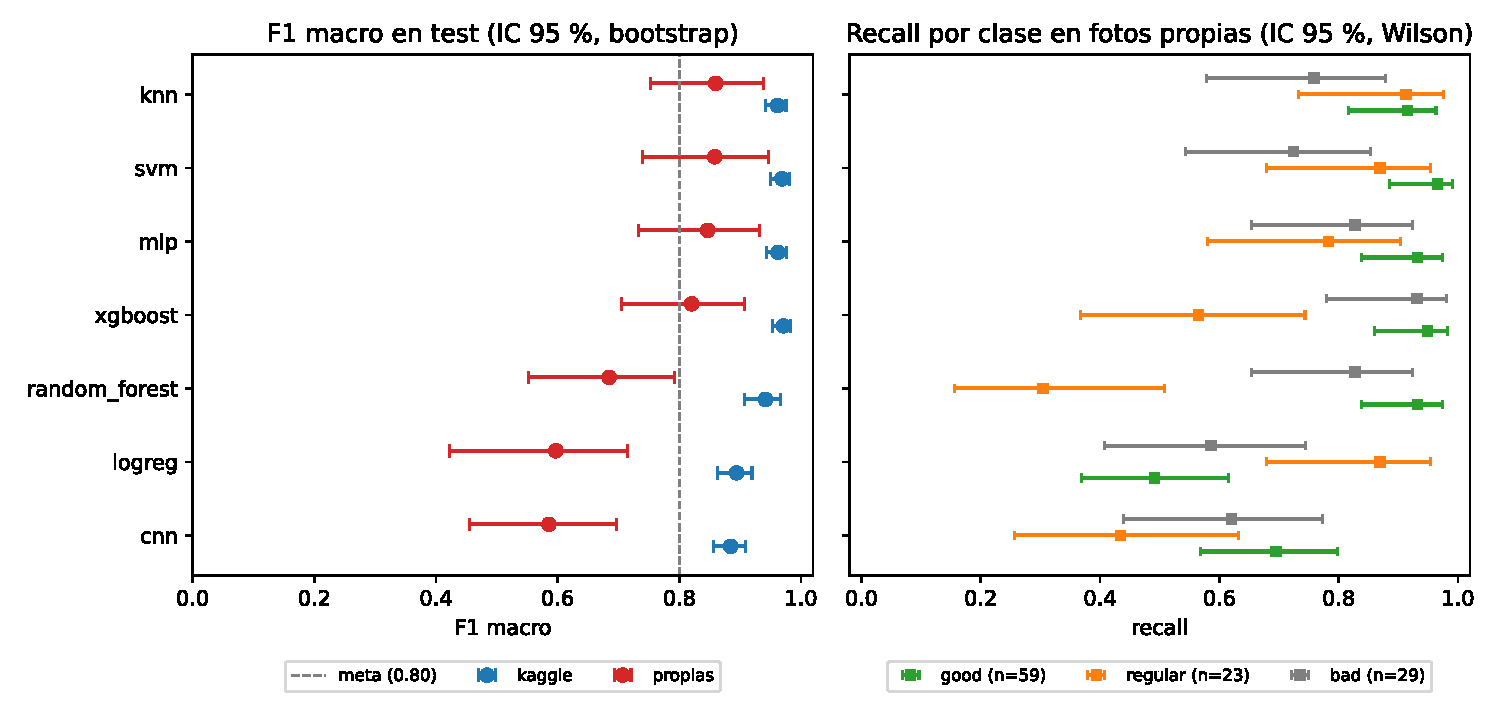
\includegraphics[width=0.78\textwidth]{figuras/ic_por_fuente.pdf}
\caption{Izquierda: F1 macro en prueba por fuente, con su intervalo de confianza del 95\,\%. Derecha: recall de cada clase en las fotos propias.}
\label{fig:ic}
\end{figure*}

KNN y SVM obtienen el F1 más alto en nuestras fotos, pero la prueba de McNemar no distingue entre KNN, SVM, MLP y XGBoost: el $p$ corregido por Holm es 1 en las seis comparaciones entre ellos. Sobre las 111 fotos, KNN falla 14 y SVM 13, y solo 8 y 7 de esos errores son de uno solo de los dos. La CNN y la regresión logística son peores que esos cuatro modelos ($p<0.001$ tras la corrección). Ningún modelo alcanza con seguridad un F1 de 0.80 en nuestras fotos, porque el límite inferior del intervalo es 0.75 para KNN y 0.74 para SVM. Con la partición anterior, que dejaba copias rotadas de una misma foto en entrenamiento y prueba, el SVM marcaba 0.88 y un recall de bad de 0.86.

Los errores del SVM en nuestras fotos se concentran en lima (5 de 13) y guayaba (4). El error más costoso para un vendedor, una fruta bad clasificada como good, aparece en 5 de las 29 bad propias, tanto en el SVM como en el KNN. XGBoost comete ese error una sola vez, pero falla en 10 de las 23 regular.

\subsection{Red convolucional}
La CNN reentrenada obtuvo un F1 de 0.74 en validación y de 0.70 en el test global: 0.88 en Kaggle y 0.59 en nuestras fotos. Reconoce menos de la mitad de las regular (recall de 0.43) y en Kaggle clasifica 98 frutas bad como good. Las curvas de entrenamiento no muestran sobreajuste: el F1 de entrenamiento, medido sin aumento de datos, es casi igual al de validación (0.79 y 0.74 en la mejor época), pero ambos suben y bajan cerca de 0.2 puntos de una época a otra. La red no memoriza; con unas 10\,400 imágenes de entrenamiento, de las que solo 180 son regular, no alcanza a aprender esa clase.

\subsection{Espacio de características}
Con PCA sobre las 62 características estandarizadas, las dos primeras componentes explican el 23.6\,\% de la varianza y hacen falta 29 para llegar al 90\,\%. La primera está dominada por la textura (LBP) y la luminosidad, y en ese plano good y bad se superponen. LDA \cite{fisher1936}, en cambio, concentra el 91\,\% de la separación entre clases en su primera dirección, que aparta good de bad (Fig.~\ref{fig:lda}). La segunda dirección separa la clase regular, pero en ella también se separan nuestras fotos de las de Kaggle. Una regresión logística entrenada solo para adivinar la fuente de cada foto a partir de las 62 características lo logra con un AUC de 0.96, incluso usando solo fotos good y bad.

\begin{figure*}[t]
\centering
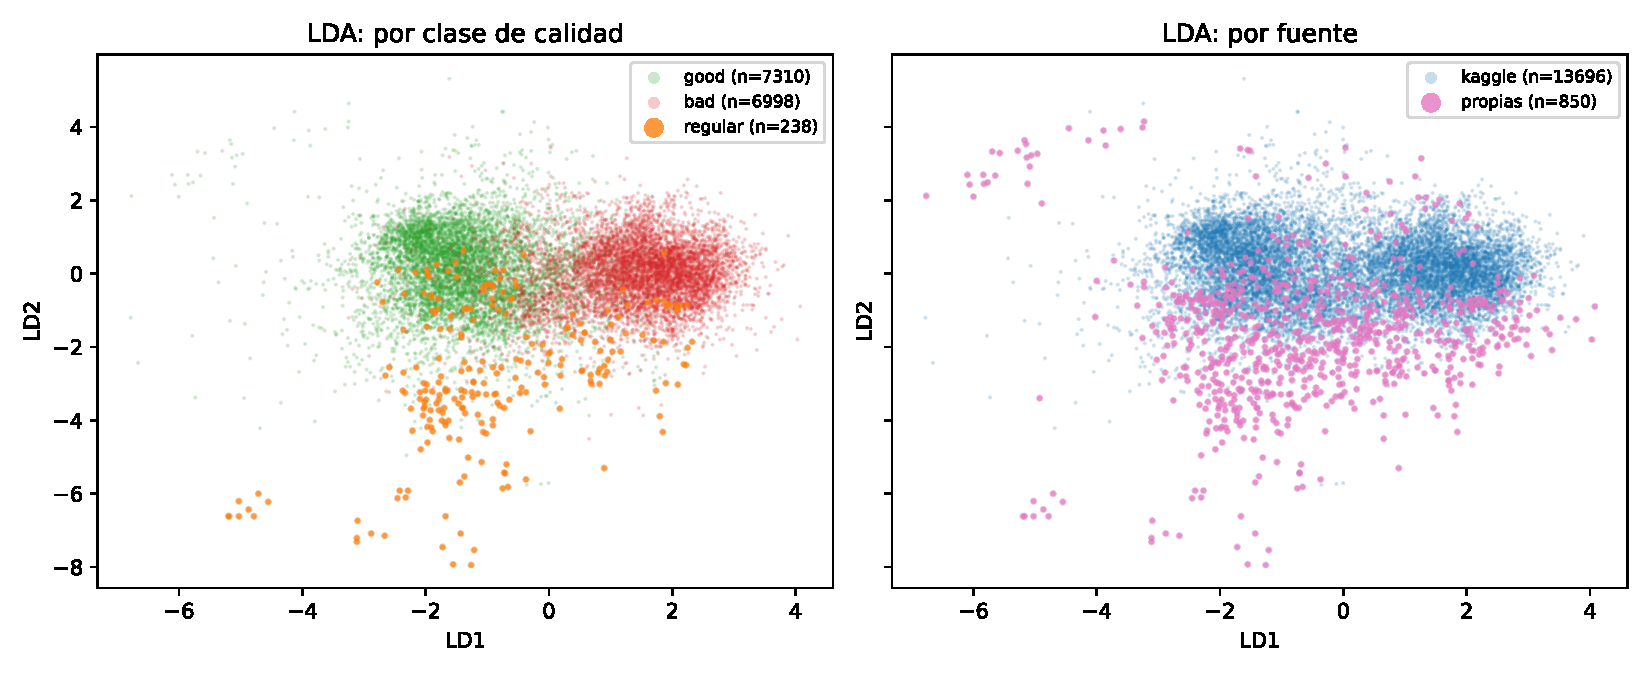
\includegraphics[width=0.78\textwidth]{figuras/lda_caracteristicas.pdf}
\caption{Proyección LDA de las 62 características, coloreada por clase (izquierda) y por fuente (derecha). La región donde está la clase regular es la misma donde están las fotos propias.}
\label{fig:lda}
\end{figure*}

\subsection{Tamaño}
La segmentación fue válida en el 87.8\,\% de las imágenes (12\,770 de 14\,546); cuando falla, la aplicación no reporta tamaño. Como las clases de tamaño salen de los terciles de $d_{norm}$, compararlas con la predicción sería circular. Medimos en cambio la repetibilidad: las fotos de un mismo grupo son la misma fruta desde otro ángulo y deberían recibir el mismo tamaño. El diámetro normalizado cambia poco dentro de cada grupo, pero la clase coincide mucho menos en nuestras fotos que en Kaggle (Tabla~\ref{tab:tamano}): basta una variación pequeña para cruzar el límite de un tercil.

\begin{table}[t]
\caption{Repetibilidad del tamaño entre fotos de la misma fruta}
\label{tab:tamano}
\centering
\footnotesize
\setlength{\tabcolsep}{3.5pt}
\begin{tabular}{lrrccc}
\toprule
Fuente & Grupos & Fotos & Acuerdo & $\kappa$ & CV de $d_{norm}$ \\
\midrule
Propias & 95 & 364 & 0.64 & 0.42 & 0.019 \\
Kaggle & 1\,208 & 6\,232 & 0.82 & 0.72 & 0.008 \\
\bottomrule
\multicolumn{6}{p{0.92\columnwidth}}{\scriptsize Acuerdo: fracción de pares de fotos del mismo grupo con la misma clase de tamaño. $\kappa$: acuerdo descontando el esperado por azar, estimado permutando las clases. CV: coeficiente de variación mediano de $d_{norm}$ dentro de cada grupo. Sin copias rotadas.}
\end{tabular}
\end{table}

\section{Análisis de resultados}
\subsection{Generalización y sobreajuste}
SVM, KNN, XGBoost, MLP y Random Forest llegan a un F1 de 0.99 o 1.00 en entrenamiento, contra 0.86 a 0.92 en validación cruzada: hay sobreajuste, aunque moderado. El F1 de validación cruzada del SVM (0.92) es igual a su F1 en el test global, así que la selección de hiperparámetros no infló la estimación. Donde la generalización falla es entre fuentes: los mismos modelos pierden entre 0.10 y 0.30 puntos al pasar de las fotos de Kaggle a las nuestras.

\subsection{Qué funciona y qué falla}
Separar good de bad funciona bien con color y textura: en Kaggle el SVM y XGBoost superan 0.96 de recall en ambas clases, y no hizo falta una red profunda para eso. La clase regular es la difícil. Es la más subjetiva, la que tiene menos ejemplos y la única que solo existe en nuestras fotos. Entre los modelos clásicos, Random Forest y XGBoost son los que más la confunden (recall de 0.30 y 0.57), y la CNN reconoce menos de la mitad. En nuestras fotos, lima y guayaba concentran la mayoría de errores del SVM. El error que más pesa en la práctica, dejar pasar una fruta bad como good, ocurre en cerca de una de cada seis bad propias con SVM y KNN.

\subsection{Cambio de dominio y aprendizaje de atajos}
La regresión logística muestra el riesgo que anticipamos: en nuestras fotos clasifica como regular 25 de las 59 good, aunque su recall de regular es alto (0.87). Como regular solo aparece en nuestras fotos, aprendió en parte a reconocer la fuente y no la calidad, un caso de aprendizaje de atajos \cite{geirhos2020}. El detector de fuente con AUC de 0.96 y la proyección LDA de la Fig.~\ref{fig:lda} muestran que las dos fuentes ocupan regiones distintas del espacio de características. Es el mismo fenómeno que reportan los bancos de prueba de cambio de distribución: un modelo con buen desempeño en su dominio pierde exactitud en otro \cite{koh2021}.

\subsection{Comparación con la literatura}
Morshed et al. \cite{morshed2022} reportan una exactitud de 99.67\,\% en FruitNet con DenseNet201 preentrenada y una partición aleatoria 60/20/20. Nuestros modelos clásicos obtienen un F1 de 0.97 en las imágenes de Kaggle con una partición agrupada, así que en ese dominio el problema está casi resuelto incluso sin redes profundas. Ese trabajo no menciona agrupar las fotos de una misma fruta; en nuestro caso, no agrupar elevó el F1 en fotos propias de 0.75 a 0.97. Tampoco evalúa con fotos de otra fuente, que es justo donde nuestros modelos pierden diez puntos o más.

\subsection{Limitaciones}
La prueba en fotos propias tiene 111 imágenes de 62 frutas físicas, y por eso los intervalos son anchos. La prueba de McNemar supone imágenes independientes, y varias fotos de una misma fruta no lo son, así que sus valores $p$ son algo optimistas. Cada foto propia la etiquetó una sola persona y no medimos el acuerdo entre anotadores. El tamaño no está calibrado en centímetros. La búsqueda de hiperparámetros de la CNN se hizo con la partición anterior y cada configuración se entrenó una sola vez. En el análisis exploratorio apareció otro caso de copias: 28 archivos que son recortes y rotaciones de solo dos fotos de banano bad, que la partición no agrupó. Por eso 4 de las 29 bad propias de prueba tienen copias en entrenamiento. Esto no cambia las conclusiones, porque el SVM falla 3 de esas 4 y XGBoost ninguna.

\section{Ética e impactos}

La Tabla~\ref{tab:etica} resume las decisiones del proyecto con implicaciones éticas, el principio del código de ética de ingeniería de software ACM/IEEE \cite{acm1999} con que se relacionan y lo que hicimos.

\begin{table}[t]
\caption{Dilemas éticos y medidas adoptadas}
\label{tab:etica}
\centering
\scriptsize
\setlength{\tabcolsep}{3pt}
\begin{tabular}{p{2.0cm}p{2.3cm}p{0.7cm}p{2.6cm}}
\toprule
Situación & Riesgo & Código & Medida \\
\midrule
Imágenes generadas con IA en la carpeta de fotos propias & Presentar datos sintéticos como reales; métricas infladas & 1.06, 3.13 & Detección por metadatos de procedencia y exclusión de las 30 imágenes \\
Clase regular solo en fotos propias & El modelo aprende la fuente y no la calidad & 3.10 & Métricas por fuente; el atajo se reporta \\
Un falso bad afecta el ingreso de un vendedor & Se descarta o se paga menos por fruta buena & 1.03, 1.04 & El sistema recomienda y una persona decide; se muestran las probabilidades \\
EXIF con GPS en el dataset público y en nuestras fotos & Revelar dónde se tomaron las fotos & 3.12, Ley 1581 & No se redistribuyen imágenes crudas; los recortes se guardan sin metadatos \\
\bottomrule
\end{tabular}
\end{table}

El análisis inicial de impactos, hecho sin resultados, está en el repositorio. La Tabla~\ref{tab:impactos} lo actualiza con lo que midieron los resultados: cada riesgo se apoya en una cifra del proyecto y cada mitigación responde a ese riesgo. La conclusión principal es que el sistema no puede decidir solo, porque en nuestras fotos los mejores modelos clasifican como good cerca de una de cada seis frutas bad. Por eso lo proponemos como apoyo a quien clasifica.

\begin{table}[t]
\caption{Matriz de impactos con la evidencia del proyecto y su mitigación}
\label{tab:impactos}
\centering
\scriptsize
\setlength{\tabcolsep}{3pt}
\begin{tabular}{p{1.15cm}p{1.9cm}p{2.25cm}p{2.3cm}}
\toprule
Dimensión & Beneficio & Riesgo y evidencia & Mitigación \\
\midrule
Social & El mismo criterio en todos los puestos; la app muestra la máscara y las probabilidades & Sensación de vigilancia si la cámara queda fija en un puesto. Seguridad del comprador: el sistema deja pasar como good 5 de 29 bad propias, y una fruta bad puede tener moho o podredumbre & La cámara encuadra solo la fruta y el fondo se borra antes de clasificar. La app no guarda imágenes. El sistema recomienda y una persona decide \\
Económica & Cuesta lo que un celular o una cámara web, no una clasificadora industrial & Un falso good genera reclamos del comprador. Un falso bad hace vender barata fruta buena: el SVM no comete ninguno en 59 good propias, el KNN comete 2 & Elegir la clase de menor costo esperado, $\hat y=\arg\min_k\allowbreak\sum_j C_{kj}\,P(j\mid\mathbf{x})$, con los costos $C_{kj}$ que fije el vendedor \\
Ambiental & La fruta regular se vende con descuento o para jugo en vez de botarse & Energía de entrenar y de clasificar en tiempo real & Modelos que corren en la CPU de un portátil (75~ms por foto); en vivo se clasifican solo 5 cuadros por segundo; parada temprana al entrenar la CNN \\
Global & El método sirve para otras frutas y otros mercados & Las variedades y las normas de calidad cambian por país: el F1 baja de 0.97 en fruta de India a 0.86 en la nuestra. Leyes de datos distintas (Ley 1581, GDPR) & Fotografiar el mercado de destino y medir el F1 por fuente antes de usar el sistema allí. Recortes sin metadatos \\
\bottomrule
\end{tabular}
\end{table}

El consumo de energía es bajo. Si suponemos que un portátil consume unos 30~W bajo carga, clasificar una foto gasta unos 2~J, y mil fotos menos de 0.001~kWh. Las ocho configuraciones de la búsqueda de la CNN tardaron en total 1.5 horas, unos 0.05~kWh. La regla de costo mínimo de la Tabla~\ref{tab:impactos} es la mitigación económica más directa. Si dejar pasar una fruta bad cuesta más que rebajar una buena, la regla exige menos probabilidad para predecir bad, y el recall de esa clase sube a costa de más falsos bad. No la aplicamos porque esos costos los debe fijar quien vende.

\section{Conclusiones y trabajo futuro}

Construimos un sistema que clasifica la calidad de una fruta en tres clases y estima su tamaño a partir de una foto, y lo evaluamos por separado con un dataset público y con fotos propias. Con características de color y textura, los mejores modelos clásicos superaron a la CNN entrenada desde cero en las dos fuentes. En nuestras fotos KNN, SVM, MLP y XGBoost quedaron estadísticamente empatados, con un F1 de 0.82 a 0.86. Las cifras cercanas a 0.97 que se obtienen con el dataset público no se trasladan a fotos tomadas en otro lugar, y la clase regular es la que más sufre.

Lo que más aprendimos fue sobre los datos. Dos veces encontramos que la forma de partir el conjunto inflaba los resultados en nuestras fotos, primero por ráfagas de fotos casi idénticas y luego por copias rotadas de una misma foto. Revisar de dónde viene cada imagen, si hay copias y si alguna es sintética cambió los resultados más que ajustar hiperparámetros. También aprendimos que, con unas decenas de fotos por clase en prueba, una diferencia de dos o tres imágenes entre modelos no dice nada si no se reporta su incertidumbre.

Como trabajo futuro proponemos: tomar más fotos bad reales, sobre todo de manzana, que solo tiene tres; etiquetar los recortes de la carpeta mixed del dataset público, para que la clase regular exista en las dos fuentes; fotografiar a distancia fija o con una moneda de referencia, para medir el tamaño en centímetros; probar aprendizaje por transferencia con una red preentrenada; calibrar el umbral de la clase bad según el costo de cada tipo de error; y medir el acuerdo entre anotadores, para saber cuánto de la confusión con la clase regular viene de las propias etiquetas.

\section*{Declaración de uso de IA}
Durante el desarrollo usamos un asistente de IA generativa (Claude, de Anthropic) como apoyo en la programación, la depuración y la redacción. Revisamos y respondemos por todo el contenido.

\begin{thebibliography}{00}
\bibitem{fao2019} FAO, \textit{The State of Food and Agriculture 2019. Moving forward on food loss and waste reduction}. Rome, Italy: FAO, 2019.
\bibitem{dnp2016} Departamento Nacional de Planeación, ``Pérdida y desperdicio de alimentos en Colombia,'' DNP, Bogotá, Colombia, 2016.
\bibitem{meshram2022} V. Meshram and K. Patil, ``FruitNet: Indian fruits image dataset with quality for machine learning applications,'' \textit{Data in Brief}, vol. 40, Art. no. 107686, 2022.
\bibitem{morshed2022} M. S. Morshed, S. Ahmed, T. Ahmed, M. U. Islam, and A. B. M. A. Rahman, ``Fruit quality assessment with densely connected convolutional neural network,'' in \textit{Proc. 12th Int. Conf. Electrical and Computer Engineering (ICECE)}, Dhaka, Bangladesh, 2022, arXiv:2212.04255.
\bibitem{otsu1979} N. Otsu, ``A threshold selection method from gray-level histograms,'' \textit{IEEE Trans. Syst., Man, Cybern.}, vol. 9, no. 1, pp. 62--66, 1979.
\bibitem{ojala2002} T. Ojala, M. Pietikäinen, and T. Mäenpää, ``Multiresolution gray-scale and rotation invariant texture classification with local binary patterns,'' \textit{IEEE Trans. Pattern Anal. Mach. Intell.}, vol. 24, no. 7, pp. 971--987, 2002.
\bibitem{haralick1973} R. M. Haralick, K. Shanmugam, and I. Dinstein, ``Textural features for image classification,'' \textit{IEEE Trans. Syst., Man, Cybern.}, vol. SMC-3, no. 6, pp. 610--621, 1973.
\bibitem{cortes1995} C. Cortes and V. Vapnik, ``Support-vector networks,'' \textit{Mach. Learn.}, vol. 20, pp. 273--297, 1995.
\bibitem{breiman2001} L. Breiman, ``Random forests,'' \textit{Mach. Learn.}, vol. 45, pp. 5--32, 2001.
\bibitem{chen2016} T. Chen and C. Guestrin, ``XGBoost: A scalable tree boosting system,'' in \textit{Proc. 22nd ACM SIGKDD Int. Conf. Knowledge Discovery and Data Mining}, 2016, pp. 785--794.
\bibitem{ioffe2015} S. Ioffe and C. Szegedy, ``Batch normalization: Accelerating deep network training by reducing internal covariate shift,'' in \textit{Proc. 32nd Int. Conf. Machine Learning (ICML)}, 2015, pp. 448--456.
\bibitem{lin2014} M. Lin, Q. Chen, and S. Yan, ``Network in network,'' in \textit{Proc. Int. Conf. Learning Representations (ICLR)}, 2014.
\bibitem{kingma2015} D. P. Kingma and J. Ba, ``Adam: A method for stochastic optimization,'' in \textit{Proc. Int. Conf. Learning Representations (ICLR)}, 2015.
\bibitem{loshchilov2017} I. Loshchilov and F. Hutter, ``SGDR: Stochastic gradient descent with warm restarts,'' in \textit{Proc. Int. Conf. Learning Representations (ICLR)}, 2017.
\bibitem{srivastava2014} N. Srivastava, G. Hinton, A. Krizhevsky, I. Sutskever, and R. Salakhutdinov, ``Dropout: A simple way to prevent neural networks from overfitting,'' \textit{J. Mach. Learn. Res.}, vol. 15, pp. 1929--1958, 2014.
\bibitem{kaufman2012} S. Kaufman, S. Rosset, C. Perlich, and O. Stitelman, ``Leakage in data mining: Formulation, detection, and avoidance,'' \textit{ACM Trans. Knowl. Discov. Data}, vol. 6, no. 4, Art. no. 15, 2012.
\bibitem{wilson1927} E. B. Wilson, ``Probable inference, the law of succession, and statistical inference,'' \textit{J. Amer. Statist. Assoc.}, vol. 22, no. 158, pp. 209--212, 1927.
\bibitem{efron1993} B. Efron and R. J. Tibshirani, \textit{An Introduction to the Bootstrap}. New York, NY, USA: Chapman \& Hall, 1993.
\bibitem{mcnemar1947} Q. McNemar, ``Note on the sampling error of the difference between correlated proportions or percentages,'' \textit{Psychometrika}, vol. 12, no. 2, pp. 153--157, 1947.
\bibitem{dietterich1998} T. G. Dietterich, ``Approximate statistical tests for comparing supervised classification learning algorithms,'' \textit{Neural Comput.}, vol. 10, no. 7, pp. 1895--1923, 1998.
\bibitem{holm1979} S. Holm, ``A simple sequentially rejective multiple test procedure,'' \textit{Scand. J. Statist.}, vol. 6, no. 2, pp. 65--70, 1979.
\bibitem{chapman2000} P. Chapman \textit{et al.}, ``CRISP-DM 1.0: Step-by-step data mining guide,'' SPSS, 2000.
\bibitem{park2024} R. Park, ``Fruit Quality Classification,'' Kaggle, 2024. [Online]. Available: \url{https://www.kaggle.com/datasets/ryandpark/fruit-quality-classification}
\bibitem{c2pa} Coalition for Content Provenance and Authenticity, ``C2PA technical specification,'' 2024. [Online]. Available: \url{https://c2pa.org/specifications/}
\bibitem{pedregosa2011} F. Pedregosa \textit{et al.}, ``Scikit-learn: Machine learning in Python,'' \textit{J. Mach. Learn. Res.}, vol. 12, pp. 2825--2830, 2011.
\bibitem{paszke2019} A. Paszke \textit{et al.}, ``PyTorch: An imperative style, high-performance deep learning library,'' in \textit{Advances in Neural Information Processing Systems 32 (NeurIPS)}, 2019, pp. 8024--8035.
\bibitem{fisher1936} R. A. Fisher, ``The use of multiple measurements in taxonomic problems,'' \textit{Ann. Eugenics}, vol. 7, no. 2, pp. 179--188, 1936.
\bibitem{geirhos2020} R. Geirhos \textit{et al.}, ``Shortcut learning in deep neural networks,'' \textit{Nature Mach. Intell.}, vol. 2, pp. 665--673, 2020.
\bibitem{koh2021} P. W. Koh \textit{et al.}, ``WILDS: A benchmark of in-the-wild distribution shifts,'' in \textit{Proc. 38th Int. Conf. Machine Learning (ICML)}, 2021, pp. 5637--5664.
\bibitem{acm1999} ACM/IEEE-CS Joint Task Force, ``Software Engineering Code of Ethics and Professional Practice,'' 1999.
\end{thebibliography}

\end{document}
